\section*{Problema P9.69}

\renewcommand*\thesection{9.69}
\numberwithin{equation}{section}

\begin{center}
    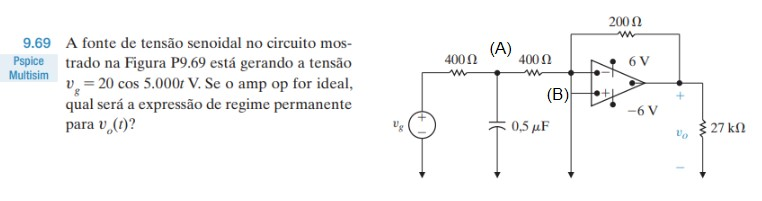
\includegraphics[scale=1.0]{P9.69.jpg}
\end{center}

O primeiro passo é expressar $V_o$ em função das tensões de entrada no AmpOp.
Aplicamos análise nodal no nó $(B)$.

\[ i_- + i_+ + \frac{V_B - V_o}{R_s} + \frac{V_B - V_A}{R_2} = 0 \]

Como o Amplificador Operacional é ideal, temos

\begin{equation}\label{eq:9.69.1}
    i_- = i_+ = 0 \un{A}
\end{equation}

Além disso, temos $V_B = 0$. Substituindo na expressão do nó, temos

\[ \frac{V_o}{R_s} + \frac{V_A}{R_2} = 0 \]

Isolando $V_o$, temos

\begin{equation}\label{eq:9.69.2}
    V_o = -\frac{R_s}{R_2} V_A
\end{equation}

Portanto, basta encontrar a expressão de $V_A$ para achar a expressão de $v_o(t)$. \\
Aplicando análise nodal no nó essencial (A), temos

\[ \frac{V_A - 20}{400} + \frac{V_A}{\frac{1}{j\omega 0,5\mu F}} + \frac{V_A - V_B}{400} = 0 \]

\[ \frac{V_A - 20}{400} + \frac{V_A}{\frac{1}{j0,0025}} + \frac{V_A}{400} = 0 \]

\[ V_A\left(\frac{1}{400} + j0,0025 + \frac{1}{400}\right) = \frac{20}{400}\]

\[ V_A = \frac{0,05}{0,005 + j0,0025} \]

\[ V_A = 8,9442\phase{-26,57^{\circ}} \un{V} \]

Assim, voltando para \eqref{eq:9.69.2}, temos

\[ V_o = -\frac{200}{400} \; 8,9442\phase{-26,57^{\circ}} \un{V} \]

\[ V_o = -4,47\phase{-26,57^{\circ}} \un{V} \]

Removendo o sinal negativo, temos

\[ V_o = 4,47\phase{-26,57^{\circ} + 180^{\circ}} \un{V} \]

\[ V_o = 4,47\phase{153,43^{\circ}} \un{V} \]

Convertendo do fasor para obter a expressão em função do tempo (note que usamos o valor de pico da tensão como o módulo do fasor),
temos

\[ \boxed{v_o(t) = 4,47\cos(5000t + 153,43^{\circ}) \un{V}}  \]











    























